%%
%% Security Testing of LLVM's Intel APX Code Generation
%% Michael Shires — University of Virginia
%% Software Security Testing, Spring 2026
%%
\documentclass[acmsmall,nonacm]{acmart}

%% Remove ACM-specific metadata blocks
\settopmatter{printacmref=false}
\renewcommand\footnotetextcopyrightpermission[1]{}
\pagestyle{plain}

\usepackage{booktabs}
\usepackage{graphicx}
\usepackage{listings}
\usepackage{xcolor}
\usepackage{multirow}

%% Tighten spacing
\setlength{\textfloatsep}{8pt plus 2pt minus 2pt}
\setlength{\floatsep}{8pt plus 2pt minus 2pt}
\setlength{\intextsep}{6pt plus 2pt minus 2pt}
\setlength{\abovecaptionskip}{4pt}
\setlength{\belowcaptionskip}{2pt}

%% Listings style for assembly
\lstdefinestyle{asm}{
  basicstyle=\ttfamily\footnotesize,
  breaklines=true,
  frame=none,
  xleftmargin=1em,
  aboveskip=0.4em,
  belowskip=0.4em,
}

\begin{document}

\title{Security Testing of LLVM's Intel APX Code Generation:\\Differential Fuzzing and Adversarial Analysis}

\author{Michael Shires}
\email{jrs6qe@virginia.edu}
\affiliation{%
  \institution{University of Virginia}
  \department{Department of Computer Science}
  \city{Charlottesville}
  \state{Virginia}
  \country{USA}
}

% ═══════════════════════════════════════════════════════════════
% ABSTRACT
% ═══════════════════════════════════════════════════════════════
\begin{abstract}
Intel Advanced Performance Extensions (APX) is the largest x86 ISA
extension in two decades, adding 16 general-purpose registers and new
instruction forms including conditional compares (CCMP), conditional
faulting moves (CFCMOV), and paired push/pop (PUSH2/POP2). Compiler
support for new ISA features is security-critical: a miscompilation
under APX-specific optimization paths can silently alter program
semantics, creating vulnerabilities invisible to source-level review.
I apply three complementary security testing methodologies to LLVM's
APX implementation: (1)~static emission analysis across 265 SPEC~CPU
2017 source files, (2)~adversarial context testing with hand-crafted
inputs targeting known compiler-fragile patterns, and (3)~IR-level
differential fuzzing of 546 randomly generated programs. I find that
LLVM's APX code generation is \emph{correct but brittle}: zero
semantic mismatches across all fuzzing campaigns, but 52\% of
adversarial test functions caused APX pattern failures. I also
identify a flag fragmentation issue where LLVM's ``full APX'' flag
(\texttt{-mapxf}) silently omits conditional faulting, leaving 1,120
CFCMOV instructions and 634 branch eliminations unrealized across
SPEC benchmarks.
\end{abstract}

\maketitle

% ═══════════════════════════════════════════════════════════════
% 1. INTRODUCTION
% ═══════════════════════════════════════════════════════════════
\section{Introduction}

Compilers are among the most trusted components in the software supply
chain. When an optimization pass silently changes what a program
computes, the result is a \emph{miscompilation}: a bug invisible to
source-level code review, static analysis, and often standard testing.
Miscompilation bugs have led to real-world security
vulnerabilities~\cite{yang2011csmith, wang2013towards}, making
compiler correctness a security-critical property.

ISA extensions are a particularly high-risk surface for
miscompilation. Each new instruction form requires new pattern-matching
logic in the compiler backend, new IR-level transformations, and new
interactions with existing optimization passes. Intel Advanced
Performance Extensions
(APX)~\cite{intel2024apx}---shipping in Granite Rapids server
processors---is the largest such extension in two decades, adding
16 registers, three-operand non-destructive instructions (NDD), paired
push/pop (PUSH2/POP2), compound conditional compares (CCMP), and
conditional faulting memory accesses (CFCMOV).

This paper applies three complementary security testing methodologies
to LLVM's APX implementation:

\begin{enumerate}
\item \textbf{Static emission analysis} across 265 SPEC~CPU~2017
  source files to quantify which APX instructions LLVM emits and
  where it leaves opportunities unrealized.

\item \textbf{Adversarial context testing} with 23 hand-crafted
  functions targeting patterns known to stress compilers: memory
  operands, volatile accesses, \texttt{setjmp/longjmp}, and complex
  control flow.

\item \textbf{Differential fuzzing} of 546 CSmith-generated programs
  compiled through three paths (no-APX, APX, APX+CF), testing whether
  APX-specific optimizations preserve program semantics.
\end{enumerate}

\noindent My key findings:

\begin{itemize}
\item \textbf{Correct but brittle.} Zero semantic mismatches across
  546 fuzzed programs, but 52\% of adversarial test functions caused
  APX patterns to silently fail.

\item \textbf{Flag fragmentation.} \texttt{-mapxf} (``full APX'')
  omits conditional faulting (\texttt{+cf}), leaving 1,120 CFCMOV
  instructions and 634 branch eliminations unrealized across SPEC.

\item \textbf{Register-only patterns.} CCMP and NDD~CMOV require
  register operands. Pointer dereferences break these
  patterns---invisible in scalar-parameter benchmarks.
\end{itemize}


% ═══════════════════════════════════════════════════════════════
% 2. BACKGROUND
% ═══════════════════════════════════════════════════════════════
\section{Background}

\subsection{Intel APX Overview}

Intel APX is a bundle of sub-features controlled by separate LLVM
feature flags (Figure~\ref{fig:hierarchy}). The user-facing flag
\texttt{-mapxf} enables four sub-features: \textbf{EGPR}
(\texttt{+egpr}, 16 new general-purpose registers r16--r31),
\textbf{NDD} (\texttt{+ndd}, three-operand non-destructive
instructions), \textbf{PUSH2/POP2} (\texttt{+push2pop2}, paired
register save/restore), and \textbf{PPX} (\texttt{+ppx}, extended
push/pop encoding). Critically, conditional faulting (\texttt{+cf}) is
\emph{not} included in \texttt{-mapxf}. This feature enables
CFCMOV---conditional memory access with hardware fault
suppression---and requires explicit opt-in via \texttt{-Xclang
-target-feature -Xclang +cf}.

\begin{figure}[t]
  \centering
  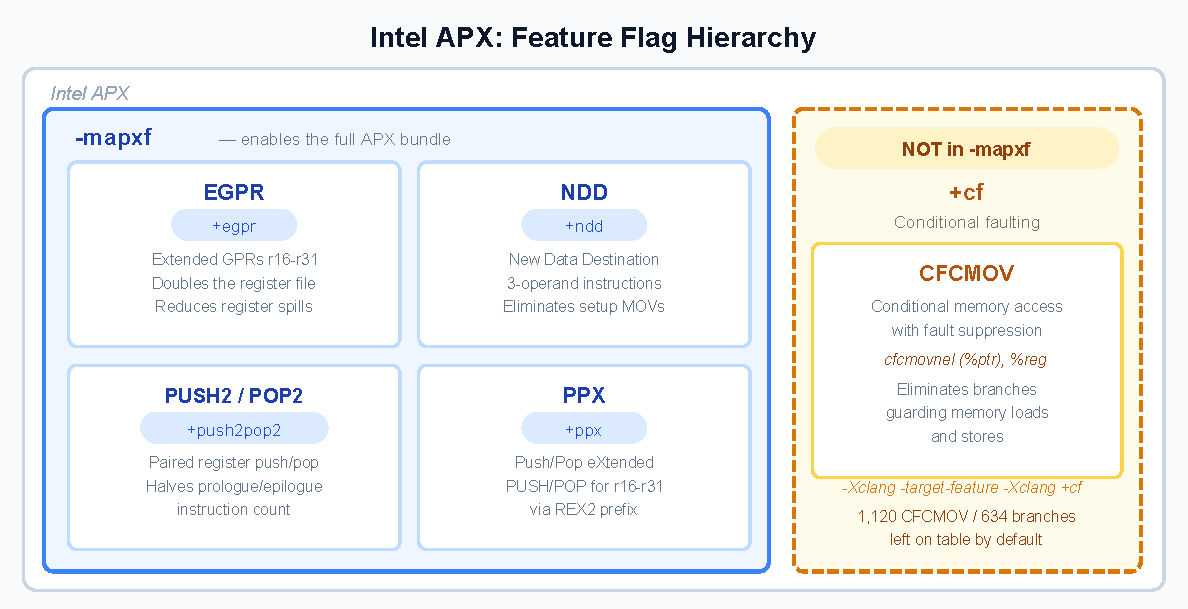
\includegraphics[width=0.85\columnwidth]{../figures/fig1_apx_hierarchy.pdf}
  \caption{APX feature flag hierarchy. \texttt{-mapxf} enables EGPR,
    NDD, PUSH2/POP2, and PPX. Conditional faulting (\texttt{+cf}),
    which gates CFCMOV, requires a separate flag.}
  \label{fig:hierarchy}
\end{figure}

\subsection{Key APX Instructions}

\textbf{CCMP} chains comparison instructions: the second comparison
executes only if the first meets a condition code, collapsing
\texttt{SETcc + AND/OR} sequences into a single chain.
\textbf{CFCMOV} performs conditional memory loads/stores with hardware
fault suppression, allowing the compiler to eliminate branches
guarding pointer dereferences. Unlike NDD~CMOV (register-to-register),
CFCMOV operates on memory operands. \textbf{PUSH2/POP2} save and
restore two callee-saved registers in a single instruction, reducing
prologue/epilogue size.

\subsection{LLVM Pipeline for APX}

APX instructions are generated at different pipeline stages:
\textbf{CFCMOV} requires an IR-level transformation where
SimplifyCFGPass replaces branch-guarded loads with
\texttt{llvm.masked.load} intrinsics \emph{before} instruction
selection. \textbf{CCMP} and \textbf{NDD~CMOV} are matched during
instruction selection (SelectionDAG). \textbf{PUSH2/POP2} are applied
during late machine-level prologue/epilogue insertion. This
distinction is security-relevant: IR-level transformations affect
\emph{all} downstream passes, while ISel-level patterns are local
substitutions.


% ═══════════════════════════════════════════════════════════════
% 3. METHODOLOGY
% ═══════════════════════════════════════════════════════════════
\section{Methodology}

\subsection{Static Emission Analysis}

I compiled 265 source files from five SPEC~CPU~2017 benchmarks
(502.gcc\_r, 505.mcf\_r, 525.x264\_r, 538.imagick\_r, 557.xz\_r)
under three configurations using clang~22.1.1: (1)~\texttt{-O2}
(baseline), (2)~\texttt{-O2 -mapxf}, and (3)~\texttt{-O2 -mapxf}
with \texttt{+cf}. I disassembled object files with
\texttt{llvm-objdump} and counted APX mnemonics. I also performed a
\emph{missed opportunity analysis}: counting compound conditional
patterns (\texttt{SETcc} chains) and \texttt{MOV+CMOV} pairs in the
baseline to measure conversion completeness.

\subsection{Adversarial Context Testing}

CSmith programs use scalar parameters---exactly where APX succeeds.
To test the boundaries, I wrote 23 functions combining APX-eligible
patterns with: memory operands (pointer dereferences), volatile
accesses, \texttt{setjmp/longjmp}, switch/computed goto, and inlining
into complex callers. Each was compiled with \texttt{-O2 -mapxf} (and
\texttt{+cf} for CFCMOV tests) and inspected for the expected APX
instruction.

\subsection{Differential Fuzzing}

\paragraph{Challenge: No APX hardware.}
APX processors were unavailable, and Intel SDE cannot run under QEMU
on Apple Silicon. I designed an \emph{IR-level differential testing}
approach that tests optimization correctness without APX hardware.

\paragraph{Three-path compilation.}
For each CSmith program: (1)~compile without APX to native x86\_64
(baseline); (2)~compile with \texttt{-mapxf} to LLVM~IR, strip APX
feature attributes, recompile to native; (3)~same as~(2) with
\texttt{+cf}. All three are executed and CSmith checksums compared.

The key insight: APX features affect optimization decisions
\emph{before} instruction selection. When \texttt{+cf} is present,
SimplifyCFGPass replaces branch-guarded loads with masked load
intrinsics---a transformation that persists after stripping feature
flags. Any semantic error (wrong condition, wrong passthrough value)
produces a different checksum.

\paragraph{Configuration.}
CSmith programs were generated with limited complexity (3~functions,
depth~2) and \mbox{\texttt{-{}-no-volatiles}}---my adversarial
testing confirmed volatile blocks all APX patterns. Fuzzing ran in
Docker (Ubuntu~24.04, x86\_64 via QEMU) with clang-19 and
CSmith~2.3.0 across two campaigns (100 + 500 programs).


% ═══════════════════════════════════════════════════════════════
% 4. RESULTS
% ═══════════════════════════════════════════════════════════════
\section{Results}

\subsection{APX Emission in SPEC~CPU~2017}

Table~\ref{tab:spec} shows APX instruction counts across five SPEC
benchmarks. PUSH2 and POP2 dominate (77.8\% of all APX instructions),
consistent with mechanical prologue/epilogue pairing. CCMP and CTEST
contribute 1,076 instructions; NDD~CMOV accounts for 847.

\begin{table}[t]
  \caption{APX instruction counts across 265 SPEC~CPU~2017 files
    (\texttt{-O2 -mapxf}, clang~22.1.1).}
  \label{tab:spec}
  \footnotesize
  \begin{tabular}{lrrrrrrr}
    \toprule
    Benchmark & Files & CCMP & CTEST & NDD & PUSH2 & POP2 & Total \\
    \midrule
    502.gcc\_r    & 38  & 129 & 89  & 173  & 609   & 663   & 1,663 \\
    505.mcf\_r    & 10  & 3   & 0   & 11   & 21    & 21    & 56    \\
    525.x264\_r   & 37  & 142 & 91  & 207  & 453   & 486   & 1,379 \\
    538.imagick\_r & 99  & 344 & 200 & 412  & 1,867 & 2,154 & 4,977 \\
    557.xz\_r     & 81  & 33  & 45  & 44   & 218   & 231   & 571   \\
    \midrule
    \textbf{Total} & \textbf{265} & \textbf{651} & \textbf{425}
      & \textbf{847} & \textbf{3,168} & \textbf{3,555} & \textbf{8,646} \\
    \bottomrule
  \end{tabular}
\end{table}

\paragraph{Conversion completeness.}
I compared APX output against non-APX patterns
(Table~\ref{tab:conversion}). CCMP achieves 105\% conversion---exceeding
the SETcc chain count because it also replaces branch-based compound
conditionals. NDD~CMOV is 100\% complete: every \texttt{MOV+CMOV}
pair (409~total) was converted. PUSH2/POP2 pairing ranges from 48--89\%,
bounded by structural constraints (odd register counts, frame pointer,
alignment) rather than compiler limitations.

\begin{table}[t]
  \caption{Conversion efficiency. CCMP exceeds 100\% by converting
    branch-based compounds beyond SETcc chains.}
  \label{tab:conversion}
  \footnotesize
  \begin{tabular}{lrrrr}
    \toprule
    Benchmark & SETcc chains & CCMP & MOV+CMOV & NDD \\
    \midrule
    502.gcc\_r    & 129 & 129 & 39  & 173 \\
    505.mcf\_r    & 0   & 3   & 2   & 11  \\
    525.x264\_r   & 195 & 142 & 63  & 207 \\
    538.imagick\_r & 253 & 344 & 289 & 412 \\
    557.xz\_r     & 45  & 33  & 16  & 44  \\
    \midrule
    \textbf{Total} & \textbf{622} & \textbf{651}
      & \textbf{409} & \textbf{847} \\
    \bottomrule
  \end{tabular}
\end{table}

\subsection{Flag Fragmentation: The Missing CFCMOV}

Recompiling with \texttt{+cf} reveals a significant gap
(Table~\ref{tab:cfcmov}): 1,120 CFCMOV instructions appear across
119 files (45\%), eliminating 634 conditional branches. Enabling
\texttt{+cf} also reduces NDD~CMOV by 66---CFCMOV subsumes cases
where a separate load plus conditional register move was needed.

\begin{table}[t]
  \caption{Impact of \texttt{+cf}. CFCMOV was entirely absent under
    the default \texttt{-mapxf}.}
  \label{tab:cfcmov}
  \footnotesize
  \begin{tabular}{lrrr}
    \toprule
    Instruction & \texttt{-mapxf} & \texttt{+cf} & $\Delta$ \\
    \midrule
    CCMP      & 651   & 656   & $+5$      \\
    CTEST     & 425   & 436   & $+11$     \\
    NDD CMOV  & 847   & 781   & $-66$     \\
    CFCMOV    & 0     & 1,120 & $\mathbf{+1{,}120}$ \\
    PUSH2/POP2 & 6,723 & 6,715 & $-8$      \\
    \midrule
    \textbf{Total} & \textbf{8,646} & \textbf{9,708} & $\mathbf{+1{,}062}$ \\
    \bottomrule
  \end{tabular}
\end{table}

The mechanism is an IR-level gate. SimplifyCFGPass queries the target
for conditional load/store support before hoisting a branch-guarded
load into a masked load intrinsic. Without \texttt{+cf}, this check
returns false and the branch persists through instruction selection.
Figure~\ref{fig:pipeline} shows the divergent paths.

\begin{figure}[t]
  \centering
  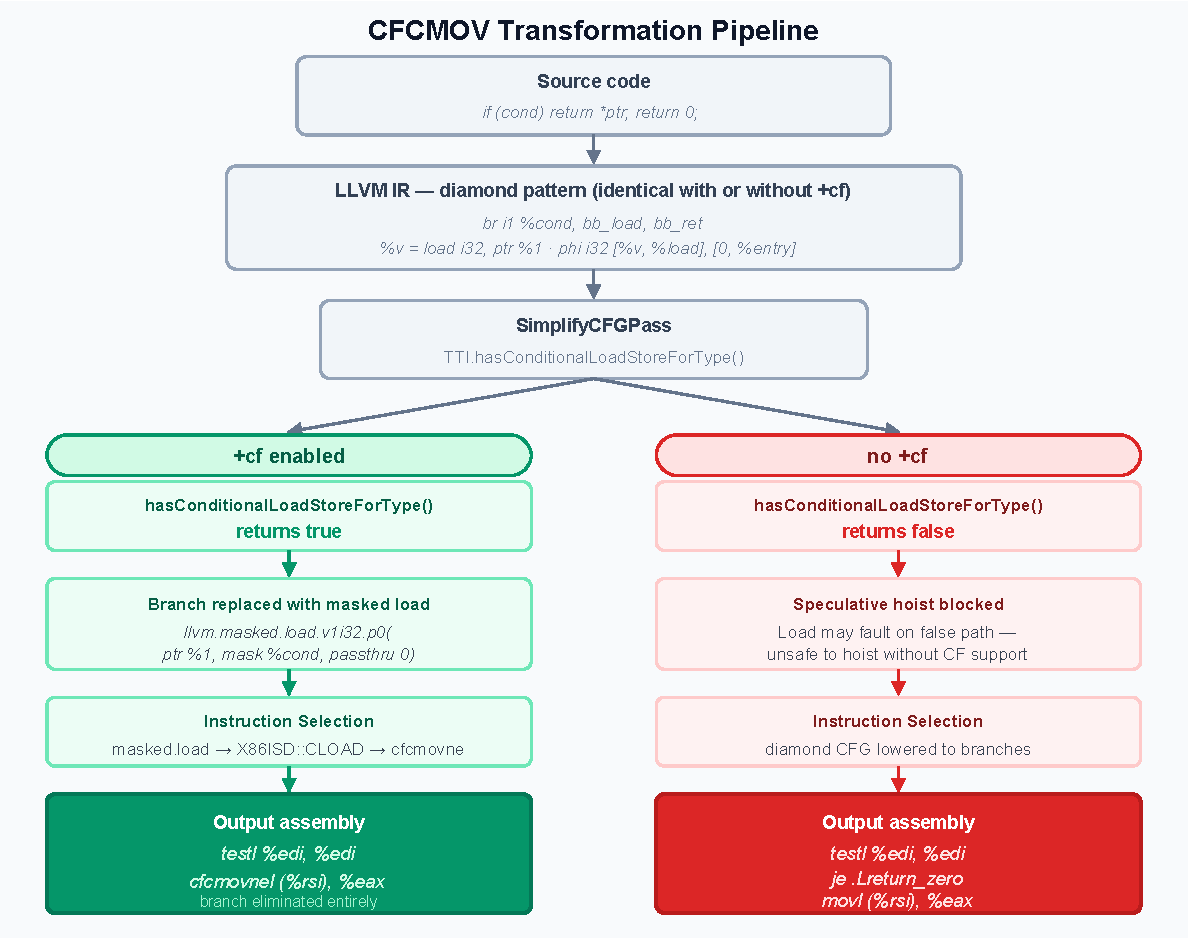
\includegraphics[width=0.65\columnwidth]{../figures/fig2_cfcmov_pipeline.pdf}
  \caption{CFCMOV pipeline. With \texttt{+cf}, SimplifyCFGPass
    replaces branch-guarded loads with \texttt{llvm.masked.load},
    eventually lowering to \texttt{cfcmovnel}. Without \texttt{+cf},
    the branch persists.}
  \label{fig:pipeline}
\end{figure}

\subsection{Adversarial Context Testing}

Figure~\ref{fig:heatmap} summarizes adversarial results: 12 of 23
functions failed to produce the expected APX instruction (52\%).

\begin{figure}[t]
  \centering
  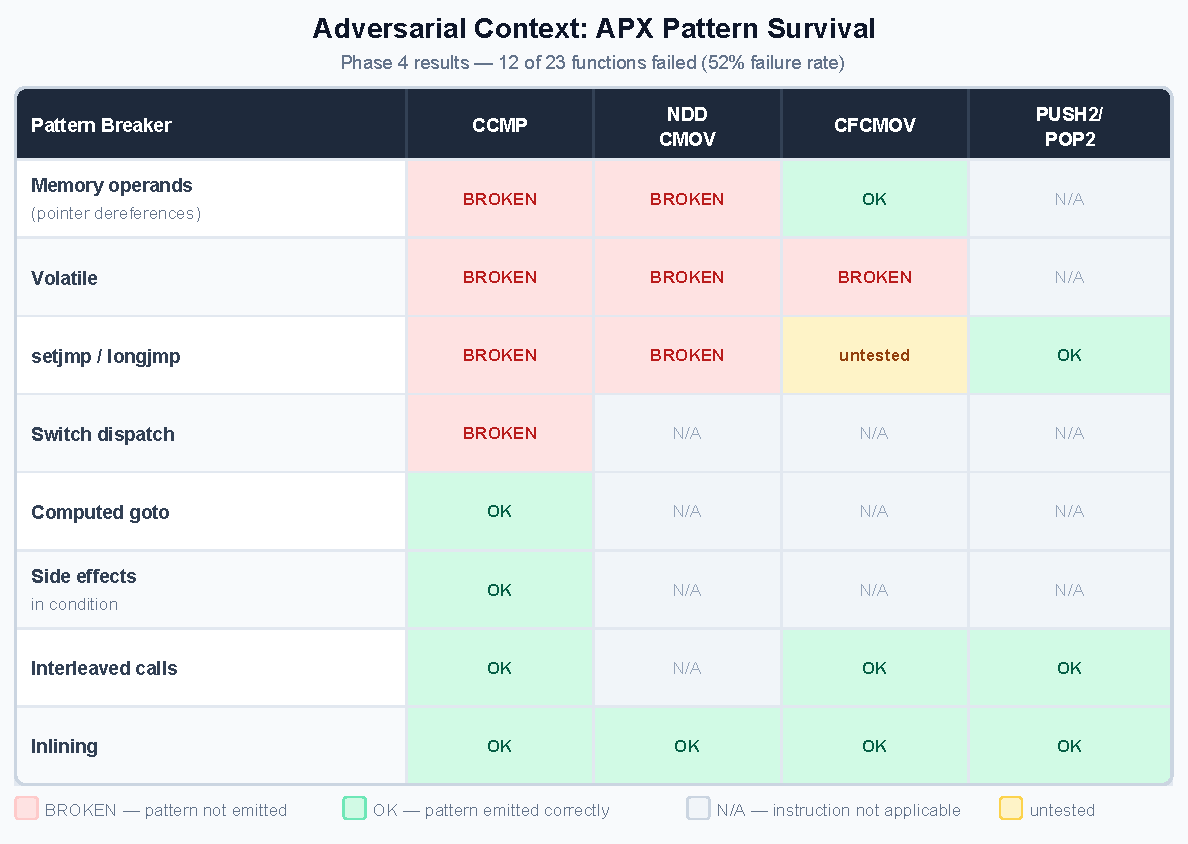
\includegraphics[width=0.78\columnwidth]{../figures/fig3_adversarial_heatmap.pdf}
  \caption{Adversarial context results. Memory operands and volatile
    break CCMP and NDD~CMOV. CFCMOV and PUSH2/POP2 are resilient.
    12/23 functions failed (52\%).}
  \label{fig:heatmap}
\end{figure}

\paragraph{Memory operands break CCMP and NDD~CMOV.}
When comparison operands are loaded via pointers, CCMP is not emitted.
Memory loads create separate basic blocks, and instruction selection
does not recognize compound conditionals across block boundaries.
Even \texttt{restrict} does not help---the issue is structural, not
alias-related.

\paragraph{Volatile blocks all APX patterns.}
Every volatile test failed. Volatile forces memory access on every
read, preventing register-based pattern matching and blocking
speculative hoisting for CFCMOV.

\paragraph{setjmp forces locals to memory.}
\texttt{setjmp} requires locals to survive non-local jumps, forcing
them to memory and killing register-based patterns. PUSH2/POP2
(prologue-level) is unaffected.

\paragraph{Resilient patterns.}
CFCMOV survived memory operand tests (its purpose \emph{is}
conditional memory access). PUSH2/POP2 survived all applicable tests.
All eight inlining test cases passed, confirming late-pipeline patterns
survive inlining into complex callers.

\subsection{Structural Impact}

APX affects basic block structure through two mechanisms. EGPR reduces
spill instructions, shrinking average block size from 6.21 to 5.78
instructions across all 265 files. CFCMOV merges previously split
blocks, raising the average slightly to 5.83 while eliminating 1,123
conditional branches ($-2.1$\%)---reducing branch predictor pressure
in compute-intensive loops.

\subsection{Differential Fuzzing Results}

Table~\ref{tab:fuzzing} shows fuzzing results. Across 546 completed
programs (100~initial + 456~extended), \textbf{zero semantic
mismatches} were detected. All three compilation paths produced
identical CSmith checksums for every completed program.

\begin{table}[t]
  \caption{Differential fuzzing: zero mismatches across 546 CSmith
    programs compiled through three paths.}
  \label{tab:fuzzing}
  \footnotesize
  \begin{tabular}{lrrr}
    \toprule
    Outcome & Initial & Extended & Combined \\
    \midrule
    Checksum match (all 3 paths) & 90  & 456 & 546 \\
    Mismatch (miscompile) & 0 & 0 & \textbf{0} \\
    Crash (APX only) & 0 & 0 & \textbf{0} \\
    \midrule
    \textbf{Programs tested} & \textbf{90} & \textbf{456} & \textbf{546} \\
    \bottomrule
  \end{tabular}
\end{table}

My IR-level approach tests optimization \emph{decisions} (SimplifyCFG
hoisting, CCMP lowering, NDD operand mapping) rather than instruction
\emph{encodings}. It does not test actual APX encoding correctness
(requiring APX hardware) or detect performance regressions.


% ═══════════════════════════════════════════════════════════════
% 5. DISCUSSION
% ═══════════════════════════════════════════════════════════════
\section{Discussion}

\paragraph{Security implications.}
LLVM does not produce \emph{wrong} APX code, but silently produces
\emph{suboptimal} code under common patterns. Branch-based conditional
memory access (without CFCMOV) is vulnerable to speculative execution
side channels; CFCMOV eliminates this vector but is silently absent
under \texttt{-mapxf}. Flag fragmentation creates a false sense of
coverage: developers reasonably expect ``full APX'' from
\texttt{-mapxf}, unaware that security-relevant optimizations require
undocumented flags.

\paragraph{Why memory operands break patterns.}
LLVM's CCMP matcher operates on register operands within a single
basic block. Memory loads may span block boundaries, and the matcher
does not recognize compound conditionals across them---even when alias
analysis confirms safety. The generated code is correct (using
branches), but CCMP's real-world effectiveness is lower than
scalar-parameter benchmarks suggest.

\paragraph{Limitations.}
I tested optimization \emph{decisions}, not APX instruction
\emph{execution} (requiring hardware or SDE). CSmith does not cover
floating-point, SIMD, or C++ exceptions. The adversarial suite is
targeted but not exhaustive.


% ═══════════════════════════════════════════════════════════════
% 6. RELATED WORK
% ═══════════════════════════════════════════════════════════════
\section{Related Work}

Yang et al.~\cite{yang2011csmith} introduced CSmith for compiler
fuzzing via differential testing. Le et al.~\cite{le2014emi} extended
this with equivalence modulo inputs (EMI). Chen et
al.~\cite{chen2016empirical} studied GCC/LLVM bugs found through
fuzzing. My work applies differential fuzzing specifically to ISA
extension code paths.

Wang et al.~\cite{wang2013towards} showed that undefined
behavior-based optimizations can introduce security vulnerabilities.
CompCert~\cite{leroy2009compcert} provides formal guarantees but does
not support APX. Alive2~\cite{lopes2021alive2} verifies LLVM~IR
transformations but does not extend to backend instruction selection.
Prior ISA extension testing has focused on
SIMD/AVX~\cite{taneja2020testing}; to my knowledge, this is the
first security-oriented characterization of LLVM's APX code
generation.


% ═══════════════════════════════════════════════════════════════
% 7. CONCLUSION
% ═══════════════════════════════════════════════════════════════
\section{Conclusion}

I applied static emission analysis, adversarial context testing, and
differential fuzzing to LLVM's Intel APX code generation. LLVM's APX
implementation is \emph{correct but incomplete}: zero semantic
mismatches across 546 fuzzed programs, but 52\% of adversarial
contexts caused silent pattern failures, and the default ``full APX''
flag leaves 1,120 conditional faulting instructions unrealized. ISA
extension support is a security-relevant compiler surface that
warrants systematic testing beyond standard regression suites.

\bibliographystyle{ACM-Reference-Format}
\bibliography{refs}

\end{document}
